\chapter{Аналитическая часть}

В данном разделе описана модель трехмерного объекта, проведена формализованная постановка задачи, рассмотрена предметная область ASCII-графики и существующие алгоритмы визуализации ASCII-графики. Также будут рассмотрены методы закраски и удаления невидимых рёбер и поверхностей, и произведён их сравнительный анализ, по итогам которого будут выбраны наиболее подходящие для решения поставленной задачи алгоритмы.

Алгоритмы визуализации теней в данной работе рассматриваться не будут, чтобы снизить вычислительную нагрузку в связи с ограниченными графическими и вычислительными возможностями целевых систем.

\section{Описание модели трехмерного объекта на сцене}

Модели задаются следующими способами~\cite{Rodgers}:
\begin{itemize}
	\item каркасная модель. В этой модели задается информация о вершинах и рёбрах объектов;
	\item поверхностная модель. Поверхность может описываться аналитически, либо может задаваться другим способом;
	\item объёмная модель. Эта форма модели отличается от поверхностной тем, что к информации о поверхности добавляется информация о том, с какой стороны расположен материал.
\end{itemize}

В данной работе будут визуализироваться трехмерные объемные объекты, в связи с чем была выбрана объёмная модель.

\section{Описание способа задания трёхмерного объекта на сцене}

Существует несколько способов задания трёхмерного объекта~\cite{Rodgers}:
\begin{itemize}
	\item аналитический способ. Этот способ характеризуется описанием объекта в неявной форме, то есть для получения визуального представления нужно вычислять значения некоторой функции в различных точках пространства;
	\item полигональная сетка. Это совокупность вершин, рёбер и граней, которые определяют форму многогранного объекта. Гранями обычно являются треугольники, так как любой полигон можно представить в виде треугольника.~\cite{Rodgers}
\end{itemize}

Для задания объектов будет использоваться полигональная сетка, так как в данной работе будут визуализироваться различные объемные объекты, включая эллипсоиды, а любая сложная поверхность или форма может быть аппроксимирована треугольниками, что делает полигональную сетку универсальным инструментом для описания объектов.

\section{Формализованная постановка задачи}

Входные данные:
\begin{itemize}
	\item описания объектов $d_1$, ..., $d_k$: объект представляется в виде полигональной сетки. Для описания требуется указать координаты вершин, нормали к каждой вершине, направленные в противоположную от поверхности сторону, и грани;
	\item информация об источниках света $ls_1$, ..., $ls_m$: белый источник света представляется в виде точечного объекта, заданного его координатами в пространстве и интенсивностью излучения;
	\item информация о наблюдателе $Z$: наблюдатель характеризуется его координатой на оси $Z$. Его взгляд всегда сонаправлен с осью $oz$, при этом ось $oy$ направлена вверх, ось $ox$ направлена влево;
    \item информация о шрифте $F$: символы ASCII, описанные векторной графикой;
    \item подмножество символов $CH=\{ch_1, ..., ch_n\}$: символы ASCII, доступные для использования
\end{itemize}

Значения коэффициента фонового освещения, диффузного освещения и зеркального освещения для объектов будут одинаковы и заданы на этапе сборки.

Возвращаемые данные:
\begin{itemize}
    \item кадр сцены, выведенный в терминал.
\end{itemize}

\begin{figure}[H]
    \centering
    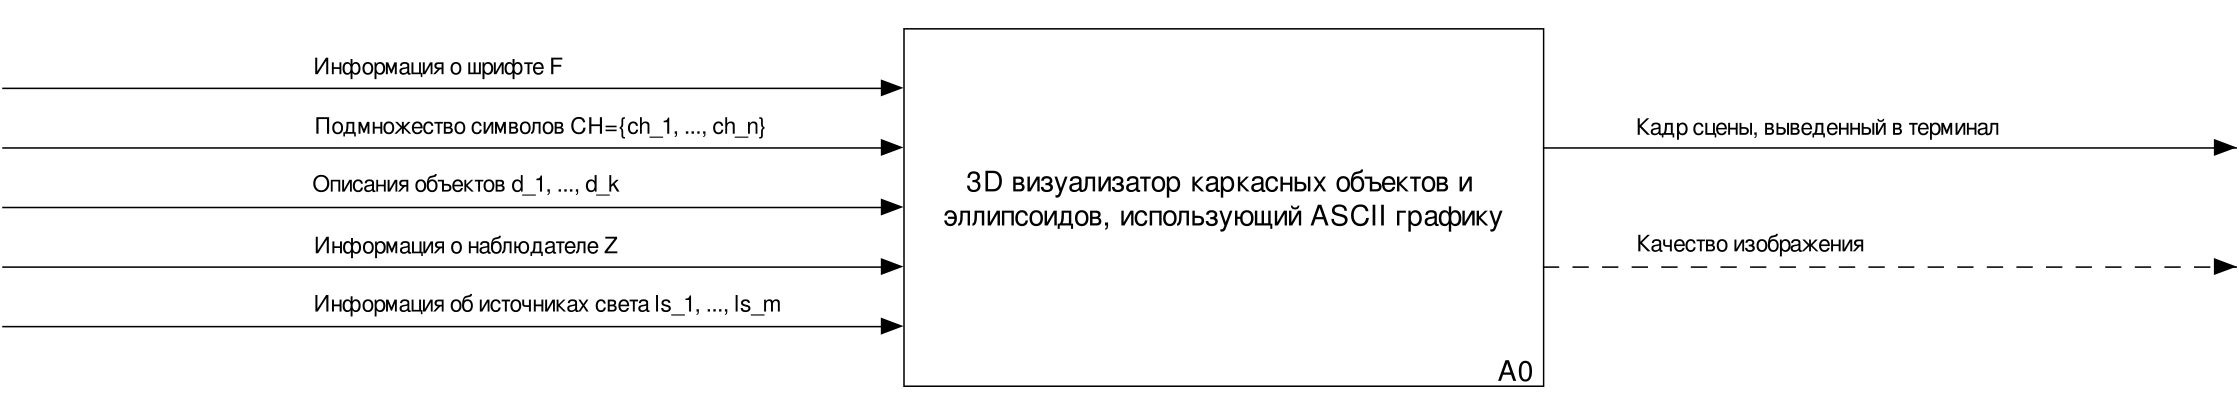
\includegraphics[scale=0.2]{images/01_A0.png}
    \caption{Формализованная постановка задачи в нотации IDEF0}
    \label{fig:idef0-0}
\end{figure}


\section{ASCII графика}

ASCII графика -- это форма визуального представления изображений и узоров, использующая знаки и символы из ASCII (American Standard Code for Information Interchange), американской стандартной кодировочной таблицы для печатных символов и некоторых специальных кодов.~\cite{ASCII-hist}

ASCII графика подразделяется на два типа, различающиеся основой:~\cite{Fast Text Placement Scheme for ASCII Art Synthesis}

\begin{itemize}
    \item яркость пикселей (пример на рис. \ref{fig:type1});
    \item форма объектов (пример на рис. \ref{fig:type2}).
\end{itemize}

\begin{figure}[H]
    \centering
    \begin{minipage}{0.45\textwidth}
        \centering
        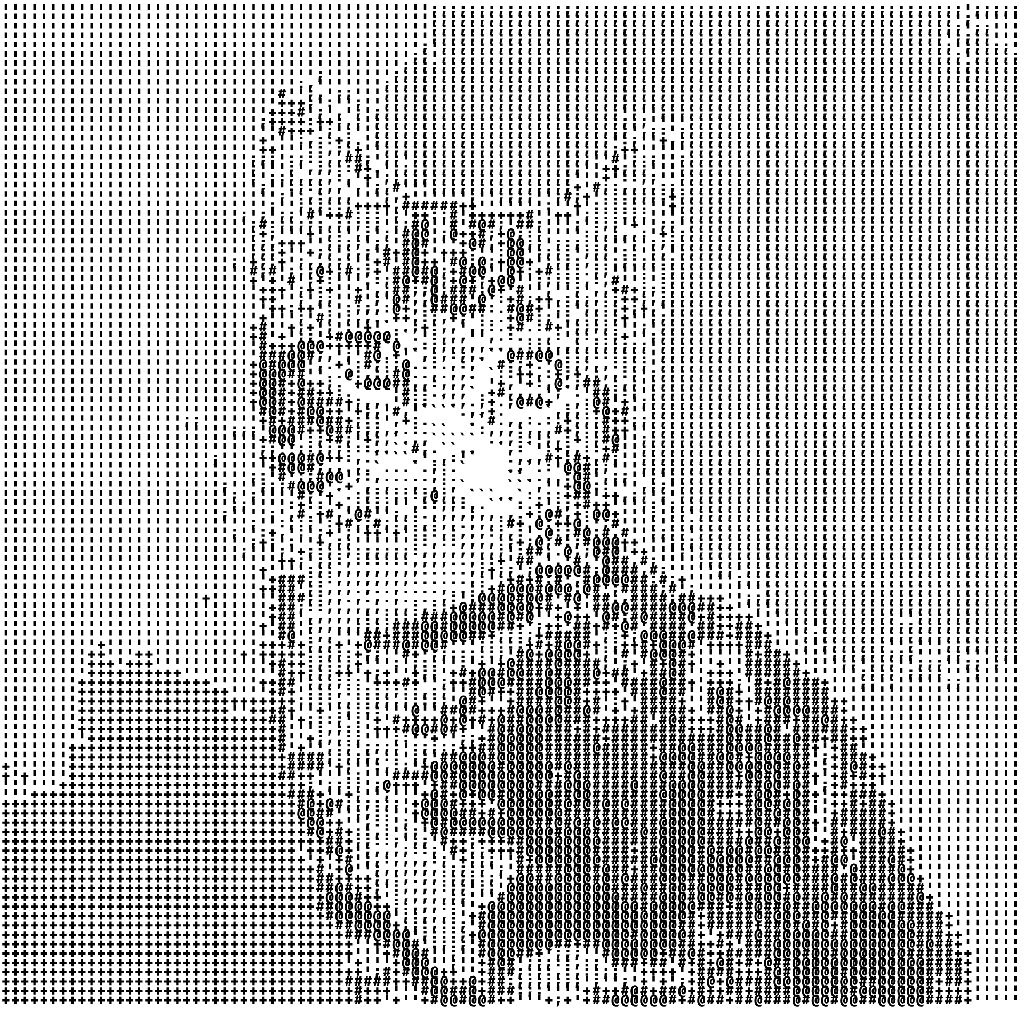
\includegraphics[width=\linewidth]{types1.png}
        \caption{}
	\label{fig:type1}
    \end{minipage}
    \begin{minipage}{0.40\textwidth}
        \centering
        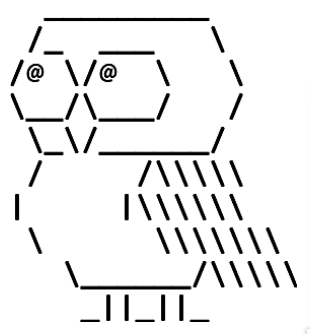
\includegraphics[width=\linewidth]{types2.png}
        \caption{}
	\label{fig:type2}
    \end{minipage}
\end{figure}

Графика, основанная на яркости пикселей, использует различные символы для представления различных уровней затенения, создавая иллюзию глубины и контраста, в то время как графика, основанная на форме, в первую очередь направлена на формирование узнаваемых контуров с использованием символов, с меньшим акцентом на тени или тон.

В данной работе планируется визуализировать как поверхности объектов, так и их грани, в связи с чем будут рассмотрены алгоритмы выбора символов ASCII для представления яркости пикселей для отрисовки поверхностей объемных объектов и алгоритмы выбора символов ASCII для представления формы для отрисовки рёбер каркасных объектов.

\section{Алгоритм выбора символов для представления формы}

Алгоритм выбора символов для представления формы будет использован для отрисовки ребер каркасных и визуальных границ эллипсоидных объектов.

Метрическая оценка сходства формы символа $ch_i$ и ячейки изображения $c_i$~\cite{Structure-based ASCII Art}:

\begin{enumerate}
    \item для $N$ выбранных точек сравниваемого символа $ch_i$ и ячейки изображения $c_i$ строятся полярные диаграммы;
    \item по полярным диаграммам строятся гистограммы, строки и столбцы которых соответствуют угловым ($Phi$) и радиальным ($R$) измерениям полярной диаграммы соответственно;
    \item $N$ полученных гистограмм представляют собой вектор $H=(h_1...h_N)$, описывающий конкретный символ или ячейку. Коэфициет $D$, используемый для оценки их сходства высчитывается по формуле (\ref{eq:StructMetric}). Чем меньше коэфициент, тем больше сходство.
\end{enumerate}

\begin{equation}
    \label{eq:StructMetric}
    D(ch_i, c_i) = \sum_{i \in N} ||H_{ch_i,i} - H_{c_i,i}||,
\end{equation}

где $ch_i$ - сравниваемый символ, $c_i$ - сравниваемая ячейка, $H_{ch_i,i}$ - i-я гистограмма вектора сравнения символа, $H_{c_i,i}$ - i-я гистограмма вектора сравнения ячейки

Пример построения гистограммы для одной из точек символа А показан на рис. (\ref{fig:StructMetric})

\begin{figure}[H]
    \centering
    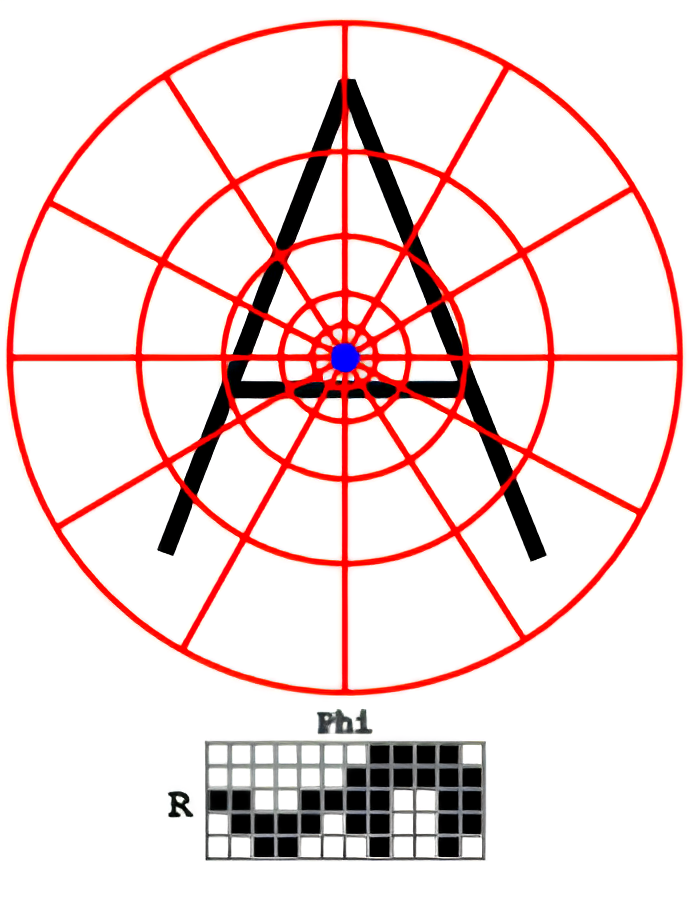
\includegraphics[scale=0.2]{StructMetric.png}
    \caption{Пример полярной диаграммы с гистограммой для одной из точек символа А}
    \label{fig:StructMetric}
\end{figure}

Для избежания многократных вычислений векторов сравнения символов, перед визуализацией объектов для всех доступных $CH$ соответствующие им вектора будут просчитаны и сохранены в карту символов по форме $MS$.

\section{Алгоритм выбора символов для представления яркости}

Алгоритм выбора символов для представления яркости будет использован для отрисовки поверхностей объемных объектов.

Составление карты доступных символов по яркости $MB$:
\begin{enumerate}
    \item отсортировать символы $CH$ по количеству пикселей, необходимых для их отображения;
    \item найти максимальное кол-во пикселей в символе $N$;
    \item рассчитать коэффициент яркости $k$ для каждого символа, где $k$ равен:
\end{enumerate}

\begin{equation}
    \label{eq:StructMetric}
    k = n_i/N, \\ 
    \text{ где } N - \text{максимальное кол-во пикселей символа},  n_i - \text{кол-во пикселей в i-м символе}
\end{equation}

Метрическая оценка сходства яркости символа $ch_i$ и ячейки изображения $c_i$~\cite{Image-to-ASCII Conversion and Preservation}:

\begin{itemize}
    \item вычисляется среднее арифметическое $avg$ яркостей пикселей ячейки $c_i$;
    \item из карты $MB$ выбирается символ, для которого разница между его коэфициентом яркости $k$ и яркостью ячейки $avg$ наименьшая.
\end{itemize}

\section{Выбор алгоритма закраски}

Для отображения поверхностей объектов необходимо использовать алгоритмы закраски. При выборе алгоритма необходимо учитывать особенности поставленной задачи. Он должен позволять отрисовывать поверхности объектов, освещённых несколькими точечными источниками света, произвольно расположенными в пространстве. Также важно учесть ограниченные вычислительные возможности целевых систем. 
Будут рассмотрены 3 основных \cite{Draw methods} алгоритма закраски:

\begin{enumerate}
	\item Простая закраска;
	\item Закраска методом Гуро;
	\item Закраска методом Фонга.
\end{enumerate}

\subsection{Простая закраска}

Вся грань закрашивается одним уровнем интенсивности, который высчитывается по закону Ламберта \cite{Rodgers}. При данной закраске все грани будут закрашены однотонно, не учитывая, под каким углом падает свет (см. рис. \ref{fig:CmpShading}). В связи с этим алгоритм не подходит для поставленной задачи.

\subsection{Закраска методом Гуро}  

Суть алгоритма заключается в интерполяции интенсивности освещения для точек внутри полигона \cite{Rodgers}.  

\begin{enumerate}  
    \item интенсивность в вершинах полигона рассчитывается по закону Ламберта, учитывая угол падения света на поверхность;
    \item для каждой точки \( P \) внутри полигона определяются барицентрические координаты относительно вершин полигона \( A \), \( B \), \( C \);
    \item используя барицентрические координаты \( \lambda_1 \), \( \lambda_2 \), \( \lambda_3 \), интенсивность в точке \( P \) вычисляется по формуле:  
    \begin{equation}
        \label{eq:int_barycentric}
        I_P = \lambda_1 \cdot I_A + \lambda_2 \cdot I_B + \lambda_3 \cdot I_C,
    \end{equation}  
    где:  
    \begin{itemize}
        \item \( \lambda_1 \), \( \lambda_2 \), \( \lambda_3 \) — барицентрические координаты точки \( P \),  
        \item \( I_A \), \( I_B \), \( I_C \) — интенсивности в вершинах \( A \), \( B \), \( C \);  
    \end{itemize}
\end{enumerate}  

Закраска методом Гуро выполняет закраску полигонов, основываясь на интерполяции интенсивности освещения, что позволяет учитывать угол падения света на поверхность (см. рис. \ref{fig:CmpShading}). Данный алгоритм подходит для поставленной задачи.

\subsection{Закраска методом Фонга}
Алгоритм работает похожим на алгоритм Гуро образом, однако ключевым отличием является то, что интерполируются не интенсивности в вершинах, а нормали~\cite{Rodgers}. Таким образом, закон Ламберта в данном алгоритме применяется в каждой точке, а не только в вершинах, что делает этот алгоритм более трудоёмким, однако позволяет учитывать кривизну поверхности.
С учётом ограниченных вычислительных возможностей целевых систем, данный алгоритм не является подходящим для поставленной задачи.

\subsection{Сравнение алгоритмов}

Визуальные различия алгоритмов закраски представлены на рисунке~\ref{fig:CmpShading}.~\cite{Gab}

\begin{figure}[H]
    \centering
    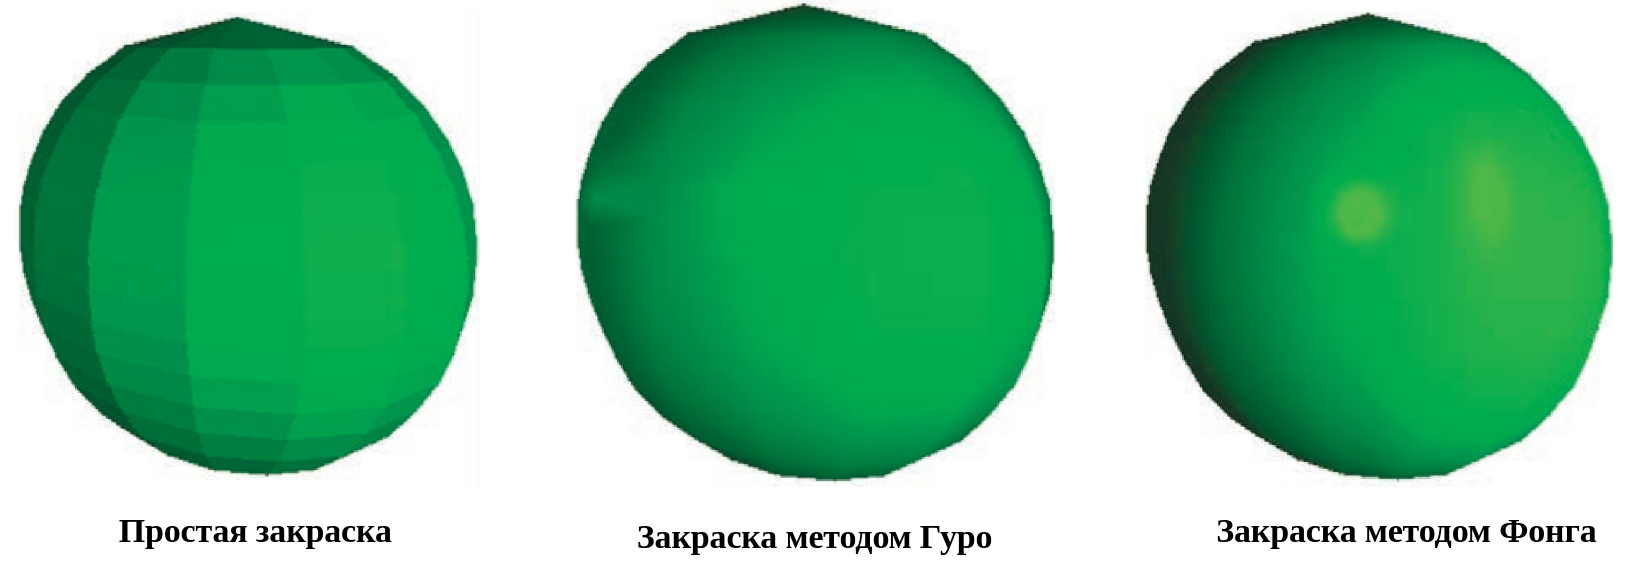
\includegraphics[scale=0.3]{CmpShading.png}
    \caption{Сравнение алгоритмов закраски}
    \label{fig:CmpShading}
\end{figure}

В таблице \ref{tbl:shading-cmp} приведено сравнение алгоритмов закраски:

\begin{table}[H]
    \centering
    \begin{tabular}{| p{5cm} | p{3cm} | p{4cm} | p{3cm} |}
    \hline
    \textbf{Критерий} & \textbf{Простая} & \textbf{Метод Гуро} & \textbf{Метод Фонга} \\
    \hline
    Количество расчетов освещения & 1 на полигон & 1 на вершину	& 1 на пиксель \\
    \hline
    Количество интерполяций & 0 & 1 (интенсивность) & 1 (нормали) \\
    \hline
    Количество операций с нормалями & 1 на полигон & 1 на вершину & 1 на пиксель \\
    \hline
    Вычислительная сложность & O(1) & $O(n_\textup{полигонов})$ & $O(n_\textup{пикселей})$ \\
    \hline
    \end{tabular}
    \caption{Сравнение методов закраски: Простая, Гуро, Фонга}
    \label{tbl:shading-cmp}
\end{table}

\subsection*{Вывод:}

Была выбрана закраска Гуро, так как он позволяет учитывать угол падения света на полигон, что делает изображение более реалистичным~\cite{Rodgers}, а также нам важна производительность, так как целевые системы обладают ограниченными вычислительными ресурсами.

\section{Выбор алгоритма удаления невидимых ребер и поверхностей}

Задача удаления невидимых рёбер в компьютерной графике заключается в том, чтобы убрать из отображения те элементы, которые не видны наблюдателю из-за их расположения или перекрытия другими объектами.

Алгоритмы удаления невидимых линий и поверхностей делятся на работающие в:
\begin{itemize}
	\item объектном пространстве (мировая система координат, высокая точность);
	\item пространстве изображений (система координат связана с дисплеем, точность ограничена разрешающей способностью дисплея).
\end{itemize}

При выборе алгоритма удаления невидимых линий необходимо учитывать особенности поставленной задачи. Важно учесть ограниченные вычислительные возможности целевых систем.
Будут рассмотрены 3 основных \cite{Invis comparison} алгоритма удаления невидимых ребер и поверхностей:

\begin{enumerate}
    \item Алгоритм Варнока;
    \item Алгоритм, использующий $Z$-буфер;
    \item Алгоритм прямой трассировки лучей.
\end{enumerate}

\subsection{Алгоритм Варнока}

Алгоритм работает в пространстве изображений и выполняет следующие шаги~\cite{Rodgers}:  

\begin{enumerate}  
    \item проверяется, является ли окно пустым или в окне содержатся только простые геометрические формы, такие как отрезки;
    \item если окно не удовлетворяет указанным условиям: разделить окно на подокна и повторить анализ содержимого для каждого подокна;
    \item повторять процесс деления до выполнения одного из условий: содержимое подокна становится достаточно простым для отображения или размер окна уменьшается до одного пикселя. 
\end{enumerate}  

\subsection{Алгоритм, использующий Z-буфер}

Данный алгоритм работает в пространстве изображения \cite{Rodgers} и выполняет следующие шаги:  

\begin{enumerate}  
    \item инициализируются два буфера:  
    \begin{itemize}  
        \item буфер кадра $I$, в котором хранятся атрибуты каждого пикселя в пространстве изображения. Размер этого буфера равен размеру изображения, то есть \( width \times height \), где \( width \) и \( height \) — размеры изображения;  
        \item $Z$-буфер, куда помещается информация о координате $z$ для каждого пикселя. Его размер также равен размеру изображения \( width \times height \), и каждый элемент хранит значение глубины для соответствующего пикселя. Изначально заполняется максимально возможными значениями глубины.
    \end{itemize}  

    \item для каждого пикселя $p$:  
    \begin{itemize}  
        \item сравнивается глубина $p$ с глубиной уже существующего в $z$-буфере.  
        \item если новый пиксель находится ближе к наблюдателю:  
        \begin{itemize}  
            \item его глубина заносится в $z$-буфер;  
            \item значение интенсивности обновляется в $I$.  
        \end{itemize}  
    \end{itemize}  
\end{enumerate}  

Основным недостатком алгоритма является значительный объем требуемой памяти для хранения двух буферов, каждый размером \( width \times height \). ~\cite{Rodgers}

\subsection{Алгоритм трассировки лучей}

Методы прямой и обратной трассировки лучей используются для моделирования траектории лучей от источника света до камеры с учётом их взаимодействия с объектами на пути.

\begin{itemize} 
    \item 
    \textbf{Прямая трассировка лучей}: Отслеживает лучи от всех источников света ко всем точкам сцены, включая те, которые не попадают в камеру, что делает метод неэффективным. \item 
    \textbf{Обратная трассировка лучей}: Более эффективный подход, отслеживающий лучи от камеры к объектам сцены и учитывающий их взаимодействие. Этот метод позволяет рассчитывать тени, отражения и преломления. Однако у него есть недостатки, такие как игнорирование вторичного освещения, высокая вычислительная сложность, резкие границы цветовых переходов и дискретность первичных лучей~\cite{Rodgers}.
\end{itemize}

\subsection{Сравнение алгоритмов}

В таблице \ref{tbl:invis-cmp} приведено сравнение алгоритмов удаления невидимых рёбер и поверхностей:

\begin{table}[H]
    \centering
    \begin{tabular}{| p{5cm} | p{3cm} | p{3cm} | p{4cm} |}
    \hline
    \textbf{Критерий} & \textbf{Варнок} & \textbf{Z-буфер} & \textbf{Трассировка лучей} \\
    \hline
    Количество операций с пикселями & Зависит от сложности сцены и деления окна & 1 на пиксель (сравнение и запись) & 1 луч на пиксель (для обратной трассировки) \\
    \hline
    Количество буферов (занимаемая память) & 1 (фреймбуфер) & 2 (фреймбуфер и Z-буфер) & Нет необходимости в дополнительных буферах \\
    \hline
    Вычислительная сложность & $O(n_\textup{подокон})$ & $O(n_\textup{пикселей})$ & $O(n_\textup{лучей})$ \\
    \hline
    \end{tabular}
    \caption{Сравнение алгоритмов: Варнока, Z-буфера, трассировки лучей}
    \label{tbl:invis-cmp}
\end{table}


\subsection*{Вывод:}

Был выбран алгоритм удаления невидимых ребер и поверхностей, использующий $Z$-буфер. Он является производительным, что делает его хорошим выбором для целевых систем.

\section{Выводы из аналитической части}
Была описана модель трехмерного объекта, проведена формализованная постановка задачи, рассмотрена предметная область ASCII-графики и существующие алгоритмы визуализации ASCII-графики.
В качестве алгоритма закраски была выбрана закраска Гуро, а в качестве алгоритма удаления невидимых рёбер и поверхностей был выбран алгоритм, использующий $Z$-буфер.

\clearpage
